\documentclass[aspectratio=169]{beamer}

% ==== Theme & basic look ====
\usetheme{Madrid}
\usecolortheme{seahorse}
\setbeamertemplate{navigation symbols}{}
\setbeamertemplate{footline}[frame number]


% Packages for mathematics  
\usepackage{amsmath}  
\usepackage{amsfonts}  
\usepackage{amssymb}  
\usepackage{graphicx}
\usepackage{bm}
\usepackage{CJKutf8}
% Support for \Tilde macro used throughout
\providecommand{\Tilde}[1]{\tilde{#1}}
\providecommand{\proofname}{Proof}
\newenvironment<>{proofs}[1][\proofname]{%
    \par
    \def\insertproofname{#1.}%
    \usebeamertemplate{proof begin}#2}
  {\usebeamertemplate{proof end}}
\makeatother

% Math shorthand and vector symbols
\newcommand{\grad}{\nabla}
\newcommand{\EE}{\mathbb{E}}
\newcommand{\dd}{\mathrm{d}}
\newcommand{\kbT}{k_B T}
\newcommand{\vx}{\mathbf{x}}
\newcommand{\mathbbm}[1]{\boldsymbol{#1}}
\newcommand{\eps}{\epsilon}
\newcommand{\z}{\mathbf{z}}
\newcommand{\vinst}{\mathbf{v}}
\newcommand{\uavg}{\overline{\mathbf{u}}}
\newcommand{\dv}[2]{\frac{d#1}{d#2}}
\newcommand{\td}{\frac{d}{dt}}
\newcommand{\x}{\mathbf{x}}
\newcommand{\coloneqq}{\mathrel{\vcenter{\baselineskip0.5ex\lineskiplimit0pt\hbox{\scriptsize.}\hbox{\scriptsize.}}}=}
\newcommand{\sg}{\mathrm{sg}}
\newcommand{\JVP}{\mathrm{JVP}}
\newcommand{\R}{\mathbb{R}}
\newcommand{\E}{\mathbb{E}}
\newcommand{\Var}{\mathrm{Var}}
\newcommand{\Cov}{\mathrm{Cov}}
\newcommand{\1}{\mathbbm{1}}
\renewcommand{\dd}{\,\mathrm{d}}
\newcommand{\pd}{\partial}
\newcommand{\given}{\,|\,}
\newcommand{\vt}{v(x,t)}
\newcommand{\vstar}{v^\star}
\newcommand{\xt}{x_t}
\newcommand{\xdot}{\dot x_t}
\newcommand{\ph}{\varphi}
\DeclareMathOperator*{\argmin}{arg\,min}
\newtheorem{remark}{Remark}
\newcommand{\Stiefel}[2]{\mathrm{St}(#1,#2)}

% Bold vector/time-indexed variables
\newcommand{\vxz}{\mathbf{x}_0}
\newcommand{\vxt}{\mathbf{x}_t}
\newcommand{\alpt}{\alpha_t}
\newcommand{\sigt}{\sigma_t}
\newcommand{\veps}{\boldsymbol{\epsilon}}
\newcommand{\vF}{\mathbf{F}}

% Title page details:   
\title[Large Foundation Models]{Large Foundation Models: Diffusion, Flow Matching, and AI for Science}  
\author{Pipi Hu}  
\institute[BIMSA]{Beijing Institute of Mathematical Sciences and Applications}  
\date{\today}  

\pgfdeclareimage[width=2cm]{logo}{../figures/logo.png}
\logo{\pgfuseimage{logo}}

% Outline slide (moved to later; avoid frame before \begin{document})

\setbeamertemplate{navigation symbols}{}
\AtBeginSection[]  
{  
    \begin{frame}<beamer>{Outline}         
        \tableofcontents[currentsection]  
    \end{frame}  
}  
  
\AtBeginSubsection[]  
{  
    \begin{frame}<beamer>{Outline}         
        \tableofcontents[currentsection,currentsubsection]  
    \end{frame}  
}  

% \setbeamertemplate{navigation symbols}{}
% \AtBeginSection[]
% {
%     \begin{frame}<beamer>{Outline}       \tableofcontents[currentsection]
%     \end{frame}
% }

\begin{document}  
  
% Title slide  
\begin{frame}  
  \titlepage  
\end{frame}  

\begin{frame}{Feynman's words}
\centering
    What I cannot create, I do not understand.
\end{frame}
  
% Presentation slides  



\section{Preliminary: Generating Samples from Probability Distributions}

\begin{frame}{Generate samples from given distribution}
Given a distribution $p(x)$, how to sample from the distribution?
\begin{itemize}
    \item Uniform distribution \& Gaussian distribution: easy sampling 
    \item Mixture Gaussian: determine which Gaussian to sample \& sample from that Gaussian
    \item A general sample function?
    \begin{itemize}
        \item \textcolor{red}{Langevin Markov Chain Monte Carlo sampling (Langevin MCMC)}
        \item Stein Variational Gradient Descent (SVGD)
        \item ...
    \end{itemize}
\end{itemize}
\end{frame}

\begin{frame}{Score function is all you need?}
A typical process of generating new samples from modeling the data distribution
    \begin{enumerate}
        \item To find the probability function $p(x)$, model $p(x;\theta)$.
        \item Normalization distribution $p(x;\theta)=\frac{1}{C(\theta)}e^{-E(x;\theta)}$ with $C(\theta)\equiv\int_x e^{-E(x;\theta)}dx$.
        \item Generating samples from above sampling methods.
    \end{enumerate}
Recall the Langevin Markov Chain Monte Carlo sampling
\begin{equation}
    x_t = x_{t-1}+\frac{\Delta t}{2}\textcolor{red}{\nabla_x\log p(x_{t-1};\theta)}+\sqrt{\Delta t}\epsilon, \quad \epsilon\sim N(0, 1).
\end{equation}
Here $\textcolor{red}{\nabla_x\log p(x_{t-1};\theta)}=-\nabla_xE(x;\theta)$ is free of the normalization $C(\theta)$.

Define the score function
\begin{equation}
    S(x;\theta) \equiv \textcolor{red}{\nabla \log p(x;\theta)}.
\end{equation}
\end{frame}

\begin{frame}{More about Langevin MCMC and the score function}
Continuous form of the Langevin MCMC
\begin{itemize}
    \item $\Delta t\to 0$
    \begin{equation}
        dx = \frac{1}{2}\nabla_x\log p(x) dt+ dB_t,
    \end{equation}
    where $dB_t$ is a Brownian motion.
    \item Given $p(x)=\frac{1}{C}e^{-E}$, we have 
    \begin{equation}
        dx = -\frac{1}{2}\textcolor{red}{\nabla_x E}dt + dB_t
    \end{equation}
\end{itemize}
Langevin MCMC is  overdamped Langevin dynamics
\begin{itemize}
    \item Langevin dynamics (MD)
    \begin{equation}
        \ddot{x} = -\nabla_x E - \gamma \dot{x} + dB_t,
    \end{equation}
    \item Given $\gamma \dot{x}
    \gg \ddot{x}$, we have the overdamped Langevin equation 
    \begin{equation}
        dx = -\frac{1}{\gamma}\nabla_x E + \frac{1}{\gamma}dB_t.
    \end{equation}
\end{itemize}
\end{frame}

\section{Matching score for training}
\begin{frame}{Matching the score by neural networks}
Recall the definition 
\begin{equation}
    S \equiv \nabla_x\log p(x),
\end{equation}
The key is to matching the score by a neural network
\begin{equation}
    J_{ESM} =\frac{1}{2} \mathbb{E}_p\left[\|s(x;\theta)-\frac{\partial \log p(x)}{\partial x}\|^2\right],
\end{equation}
where $J_{ESM}$ is called Explicit Score Matching loss. However, it is not tractable to compute $\frac{\partial \log p(x)}{\partial x}$ from data.\\[1em]

Where should we go?
\end{frame}

\begin{frame}{Implicit Score Matching (ISM) loss}
Implicit Score Matching loss (Aapo, 2005) was developed to make a tractable score matching 
\begin{equation}
    J_{ISM} \equiv \mathbb{E}_p\left[\frac{1}{2}\|s(x;\theta)\|^2+\nabla\cdot s(x;\theta)\right]=J_{ESM}-C.
\end{equation}
\end{frame}

\begin{frame}{ISM Proof: Expansion of ESM}
\begin{proof}
First, we expand the ESM loss:
\begin{equation}
    J_{ESM}=\frac{1}{2} \mathbb{E}_p\left[\|s(x;\theta)-\frac{\partial \log p(x)}{\partial x}\|^2\right]
\end{equation}
\begin{equation}
    = \frac{1}{2} \mathbb{E}_p\left[\|s\|^2\right]- \mathbb{E}_p[s\cdot\frac{\partial \log p}{\partial x}] + \frac{1}{2}\mathbb{E}_p\left[\|\frac{\partial \log p}{\partial x}\|^2\right]
\end{equation}
The key insight is to simplify the cross term using integration by parts.
\end{proof}
\end{frame}

\begin{frame}{ISM Proof: Integration by Parts}
\begin{proofs}[\proofname\ (Cont)]
The cross term can be simplified:
\begin{equation}
    -  \mathbb{E}_p[s\cdot\frac{\partial \log p}{\partial x}] =-\int_x ps\cdot \nabla \log p dx
\end{equation}
\begin{equation}
    = -\int_x ps\cdot \frac{\nabla p}{p}dx = -\int_x s\cdot \nabla pdx
\end{equation}
\begin{equation}
    = -\int \nabla\cdot(ps)dx + \int p\nabla\cdot sdx=\mathbb{E}_p[\nabla\cdot s]
\end{equation}
\end{proofs}
\end{frame}

\begin{frame}{ISM Proof: Final Result}
\begin{proofs}[\proofname\ (Cont)]
Therefore, we have:
\begin{equation}
    J_{ISM}= J_{ESM}-C
\end{equation}
where $C \equiv \frac{1}{2}\mathbb{E}_p\left[\|\frac{\partial \log p}{\partial x}\|^2\right]$ is a constant independent of $\theta$.

This makes ISM tractable since we don't need to compute the true score function.
\end{proofs}
\end{frame}

\begin{frame}{Denoising Score Matching (DSM) loss}
However, the ISM score is not very stable to optimize, with two reasons
\begin{enumerate}
    \item Expectation is performed on the whole distribution;
    \item The loss is negative decreasing to $-C$ with a great quantity, e.g. $-1e5$.
\end{enumerate}

Denoising Score Matching (DSM) loss (Vincent, 2011) is developed to solve this problem
\begin{equation}
    J_{DSM} = \frac{1}{2}\mathbb{E}_{p(x,\Tilde{x})}\left[\|s(\Tilde{x};\theta)-\nabla_{\Tilde{x}}\log p(\Tilde{x}|x)\|^2\right].
\end{equation}
And we can prove that $J_{DSM} = J_{ESM}+C$.
\end{frame}

\begin{frame}{DSM Proof: Expansion}
\begin{proof}
We expand the DSM loss:
\begin{equation}
    J_{DSM} \equiv \frac{1}{2}\mathbb{E}_{p(x,\Tilde{x})}\left[\|s(\Tilde{x};\theta)-\nabla_{\Tilde{x}}\log p(\Tilde{x}|x)\|^2\right]
\end{equation}
\begin{equation}
    =\frac{1}{2}\mathbb{E}_{p(\Tilde{x})}\left[\|s(\Tilde{x})\|^2\right]-\mathbb{E}_{p(x,\Tilde{x})}[s(\Tilde{x})\cdot\nabla_{\Tilde{x}}\log p(\Tilde{x}|x)]
\end{equation}
\begin{equation}
    +\frac{1}{2}\mathbb{E}_{p(x,\Tilde{x})}[\|\nabla_{\Tilde{x}}\log p(\Tilde{x}|x)\|^2]
\end{equation}
The key step is to show that the cross terms of $J_{ESM}$ and $J_{DSM}$ are equal.
\end{proof}
\end{frame}

\begin{frame}{DSM Proof: Cross Term Equivalence}
\begin{proofs}[\proofname\ (Cont)]
We need to show:
\begin{equation}
    \mathbb{E}_p(\Tilde{x})[s(\Tilde{x})\cdot\nabla_{\Tilde{x}}\log p(\Tilde{x})] = \mathbb{E}_{p(\Tilde{x},x)}\left[s(\Tilde{x})\cdot\nabla_{\Tilde{x}} \log p(\Tilde{x}|x)\right]
\end{equation}
Starting from the left side:
\begin{equation}
    = \int_{\Tilde{x}} p(\Tilde{x})s(\Tilde{x})\cdot\nabla_{\Tilde{x}}\log p(\Tilde{x})d\Tilde{x}
\end{equation}
\begin{equation}
    = \int_{\Tilde{x}} s(\Tilde{x})\cdot\nabla_{\Tilde{x}} p(\Tilde{x})d\Tilde{x}
\end{equation}
\end{proofs}
\end{frame}

\begin{frame}{DSM Proof: Cross Term Equivalence (Cont)}
\begin{proofs}[\proofname\ (Cont)]
Continuing the derivation:
\begin{equation}
    = \int_{\Tilde{x}}\int_x p(x)s(\Tilde{x})\cdot\nabla_{\Tilde{x}} p(\Tilde{x}|x)d\Tilde{x}dx
\end{equation}
\begin{equation}
    = \int_{\Tilde{x}}\int_x p(\Tilde{x}|x)p(x)s(\Tilde{x})\cdot\nabla_{\Tilde{x}} \log p(\Tilde{x}|x)d\Tilde{x}dx
\end{equation}
\begin{equation}
    = \mathbb{E}_{p(\Tilde{x},x)}\left[s(\Tilde{x})\cdot\nabla_{\Tilde{x}} \log p(\Tilde{x}|x)\right]
\end{equation}
This completes the proof of cross term equivalence.
\end{proofs}
\end{frame}

\begin{frame}{DSM Proof: Final Result}
\begin{proofs}[\proofname\ (Cont)]
Therefore, we have:
\begin{equation}
    J_{DSM} = J_{ESM} -\frac{1}{2}\mathbb{E}_p\left[\|\nabla_{\Tilde{x}} \log p(\Tilde{x})\|^2\right] + \frac{1}{2}\mathbb{E}_{p(x,\Tilde{x})}[\|\nabla_{\Tilde{x}}\log p(\Tilde{x}|x)\|^2]
\end{equation}
Since the last two terms are constants independent of $\theta$, we have $J_{DSM} = J_{ESM} + C$ where $C$ is a constant.
\end{proofs}
\end{frame}

\begin{frame}{DSM is all you need?}
Problem arises when $\Tilde{x}\to x$. 
We can prove that when Gaussian noised added by  $p(\Tilde{x}|x) = N(\alpha x, \sigma^2)$, 
\begin{equation}
    J_{DSM}\to \infty, \text{ if } \Tilde{x}\to x.
\end{equation}
\begin{proof}
  Given the Gaussian noise added, we have \\[-1em] 
  \begin{equation}
\nabla_{\Tilde{x}}\log p(\Tilde{x}|x) = \nabla_{\Tilde{x}}\log e^{-\frac{(\Tilde{x}-\alpha x)^2}{2\sigma^2}} = -\frac{\Tilde{x}-\alpha x}{\sigma^2}.
  \end{equation}  
And we can show that the following formula goes to infinity\\[-1em]
\begin{equation}
\begin{aligned}
&\mathbb{E}_{p(x,\Tilde{x})}[\|\nabla_{\Tilde{x}}\log p(\Tilde{x}|x)\|^2] 
=\mathbb{E}_{p(x,\Tilde{x})}[\|\frac{\Tilde{x}-\alpha x}{\sigma^2}\|^2]\\
&=\mathbb{E}_{p(x)}\mathbb{E}_{p(\Tilde{x}|x)}[\|\frac{\Tilde{x}-\alpha x}{\sigma^2}\|^2]
=\mathbb{E}_{\epsilon\sim N(0,1)}[\|\frac{\epsilon}{\sigma}\|^2] \to \infty \text{ if } \sigma\to 0.
\end{aligned}
\end{equation}
Finally, we know that\\[-1em]
\begin{equation}
    J_{DSM} = J_{ESM}+C \to \infty \text{ as } C\to \infty \text{ when } \Tilde{x}\to x.
\end{equation}
\end{proof}  
\end{frame}

\section{Relations of different models: x0, epsilon and score model}

\begin{frame}{Revisit the adding noise from $x$ to $\Tilde{x}$}
Gaussian transition kernel for adding noise from $x$ to $\Tilde{x}$
\begin{equation}
    \Tilde{x} = \alpha x + \sigma \epsilon,
\end{equation}
which equivalent to the Gaussian transition kernel
\begin{equation}
    p(\Tilde{x}|x) = N(\Tilde{x}; \alpha x, \sigma^2),
\end{equation}
where $\epsilon\sim N(0,1)$ and 
\begin{equation}
    N(\Tilde{x};\alpha x, \sigma^2) = C e^{-\frac{\|\Tilde{x}-\alpha x\|^2}{2\sigma^2}}.
\end{equation}
And 
\begin{equation}
    \epsilon = \frac{\Tilde{x}-\alpha x}{\sigma}.
\end{equation}\\[1em]

Questions arise: how can we get $x$ given $\Tilde{x}$?
\end{frame}

\begin{frame}{Tweedie's Formula}
    Tweedie's Formula (Bayes statistics) states (Robbins, 1956)
    \begin{theorem}
        Given random variables $x, y$, $y\sim N(x, \sigma^2I)$, i.e., $p(y|x) = N(x, \sigma^2)$, the expectation of $x$ could be given by 
        \begin{equation}
            \mathbb{E}[x|y] = y +\textcolor{red}{\sigma^2}\nabla \log p(y).
        \end{equation}
    \end{theorem}

Let
\begin{equation}
   x \leftarrow \alpha x, \quad y \leftarrow \Tilde{x},
\end{equation}
we have 
\begin{equation}
    s\equiv \nabla_{\Tilde{x}} \log p(\Tilde{x}) = -\frac{\Tilde{x}-\alpha \mathbb{E}[x|\Tilde{x}]}{\sigma^2}= -\frac{1}{\sigma}\mathbb{E}[\frac{\Tilde{x}-\alpha x}{\sigma}|\Tilde{x}] = -\frac{\mathbb{E}[\epsilon|\Tilde{x}]}{\sigma},
\end{equation}
where we have used the fact
$\epsilon = \frac{\Tilde{x}-\alpha x}{\sigma}.$

\end{frame}

\begin{frame}{Another insight: from the definition of the score $S$}
    Recall that adding noise by
    $\Tilde{x} = \alpha x + \sigma \epsilon$,
\begin{equation}\label{eq:cond}
    p(\Tilde{x}|x) = Ce^{-\frac{\|\Tilde{x}-\alpha x\|^2}{2\sigma^2}}.
\end{equation}
Hence
\begin{equation}
    s(\Tilde{x}) = \nabla_{\Tilde{x}}\log p(\Tilde{x}) = \frac{\nabla_{\Tilde{x}}p(\Tilde{x})}{p(\Tilde{x})}=\frac{\int_x \nabla_{\Tilde{x}}p(\Tilde{x}|x) p(x)dx}{p(\Tilde{x})},
\end{equation}
From Eq. \eqref{eq:cond}, we have
\begin{equation}
s(\Tilde{x}) = \frac{\int_x \nabla_{\Tilde{x}} \log p(\Tilde{x}|x)p(\Tilde{x}|x) p(x)dx}{p(\Tilde{x})} = \int_x \nabla_{\Tilde{x}} \log p(\Tilde{x}|x)p(x|\Tilde{x})dx, 
\end{equation}
leading to
\begin{equation}
s(\Tilde{x}) = \mathbb{E}_x[\nabla_{\Tilde{x}} \log p(\Tilde{x}|x)| \Tilde{x}]=\mathbb{E}_x[-\frac{\Tilde{x}-\alpha x}{\sigma^2}| \Tilde{x}] = -\frac{\Tilde{x}-\alpha \mathbb{E}[x|\Tilde{x}]}{\sigma^2}.
\end{equation}
\end{frame}

\begin{frame}{Theoretical Support: Conditional Expectation}
\begin{theorem}
\label{thm:conditional_expect}
    Let $X$ be an integrable random variable. Then for each $\sigma$-algebra $\mathcal{V}$ and $Z \in \mathcal{V}$, $Z^* = \mathbb{E}(X| \mathcal{V})$ solves the least square problem %\cite{evans2012introduction}
    $$\text{argmin}_{Z\in \mathcal{V}} \| Z - X\|\,,$$
    where $\| Z\| = \left( \int Z^2 dP \right)^{\frac{1}{2}}$.
\end{theorem}

\begin{figure}
    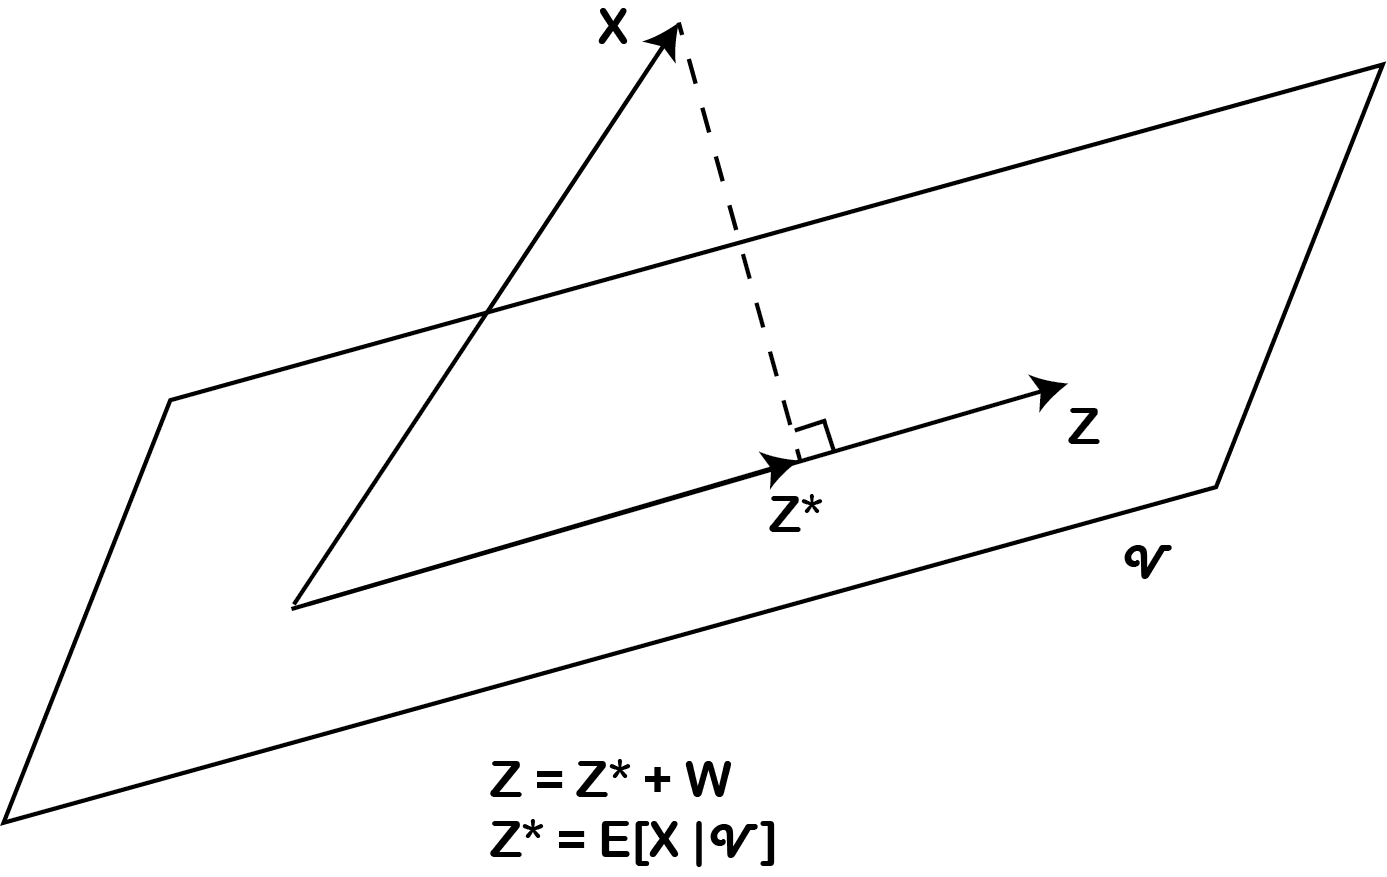
\includegraphics[width=0.4\textwidth]{../figures/conditional_expectation.png}
\end{figure}
\end{frame}

\begin{frame}{Setting}
    Let $(\Omega,\mathcal F,\mathbb P)$ be a probability space and $L^2:=L^2(\Omega,\mathcal F,\mathbb P)$ with
    $\langle U,V\rangle=\mathbb E[UV]$.  
    Fix a sub-$\sigma$-field $\mathcal G\subset\mathcal F$ and denote the closed subspace
    \[
    \mathcal V:=L^2(\mathcal G)=\{Z\in L^2: Z \text{ is }\mathcal G\text{-measurable}\}.
    \]
    \textbf{Claim.} For $X\in L^2$,
    \[
    Z^*:=\mathbb E[X\mid\mathcal G]\in\mathcal V
    \quad\text{and}\quad
    Z^*=\arg\min_{Z\in\mathcal V}\ \mathbb E[(Z-X)^2].
    \]
    \end{frame}

    \begin{frame}{Proof of the claim}
    For any $Z\in\mathcal V$,
    \[
    \langle X-Z^*, Z\rangle
    =\mathbb E\!\left[(X-Z^*)Z\right]
    =\mathbb E\!\left(\mathbb E[(X-Z^*)Z\mid\mathcal G]\right)
    =\mathbb E\!\left(Z\,\mathbb E[X-Z^*\mid\mathcal G]\right)=0.
    \]
    Hence $X-Z^*\perp\mathcal V$.
    \vspace{1em}
 
    Let any $Z\in\mathcal V$ be written as $Z=Z^*+W$ with $W\in\mathcal V$. Then
    \[
    \|X-Z\|_2^2=\|X-(Z^*+W)\|_2^2
    =\|X-Z^*\|_2^2+\|W\|_2^2
    \ge \|X-Z^*\|_2^2,
    \]
    because $\langle X-Z^*,W\rangle=0$.  
    Equality $\Leftrightarrow W=0 \Leftrightarrow Z=Z^*$, proving uniqueness and the minimizer claim.
\end{frame}


\begin{frame}{Revisit several models}
\begin{enumerate}
    \item Score model 
    \begin{equation}
        Loss_{score} = \|s_\theta(\Tilde{x}) - \frac{\epsilon}{\sigma}\|^2;
    \end{equation}
    \item $X$ prediction model ( denoising model, $x0$ model)
    \begin{equation}
        Loss_{x_0} = \|x_\theta (\Tilde{x})-x\|^2,
    \end{equation}
    with 
    \begin{equation}
        s(\Tilde{x}) = -\frac{\Tilde{x}-\alpha x_{\theta^*} (\Tilde{x})}{\sigma^2}
    \end{equation}
    where $x_\theta(\Tilde{x}) \to x_{\theta^*}(\Tilde{x})\equiv \mathbb{E}[x|\Tilde{x}]$;
    \item $\epsilon$ prediction model
    \begin{equation}
        Loss_{\epsilon} = \|\epsilon_\theta(\Tilde{x})-\epsilon\|^2,
    \end{equation}
    with
    \begin{equation}
        s(\Tilde{x}) = -\frac{\epsilon_{\theta^*}(\Tilde{x})}{\sigma},
    \end{equation}
    where $\epsilon_\theta(\Tilde{x})\to\epsilon_{\theta^*}(\Tilde{x})\equiv\mathbb{E}[\epsilon|\Tilde{x}]$.
\end{enumerate}
\end{frame}

\begin{frame}{The consistency of the three modeling}

As stated before, we have the following connection in the optimal $(\theta^*)$ case
\begin{equation}
    s_{\theta^{*}}(\Tilde{x}) = -\frac{\Tilde{x}-\alpha x_{\theta^*} (\Tilde{x})}{\sigma^2} =  -\frac{\epsilon_{\theta^*}(\Tilde{x})}{\sigma},
\end{equation}
by the above conditional expectation. 

Hence, in the real modeling of designing the loss, we use the connection of three models without reaching the optimal parameter
\begin{equation}
    s_\theta(\Tilde{x}) = -\frac{\Tilde{x}-\alpha x_{\theta} (\Tilde{x})}{\sigma^2} =  -\frac{\epsilon_{\theta}(\Tilde{x})}{\sigma},
\end{equation}
and substitute each other form to the loss definition above, we can recover all of the losses given by different models.
\end{frame}


\section{Potential Score Matching loss}
% ============================================================
\begin{frame}{Key Identity: Jacobian Switch (chain rule between $\vx_0$ and $\vx_t$)}
    The Gaussian transition density is
    \[
    q(\vxt\mid \vxz) = \mathcal{N}\!\big(\vxt;\; \alpt\,\vxz,\, \sigt^2\mathbf{I}\big) \propto \exp\!\Big(-\tfrac{\|\vxt-\alpt\,\vxz\|^2}{2\sigt^2}\Big).
    \]
    A basic but crucial identity:
    \[
    \grad_{\vxt} q(\vxt\mid \vxz) = -\frac{1}{\alpt}\,\grad_{\vxz} q(\vxt\mid \vxz),\qquad (\alpt>0).
    \]
    \textbf{Proof sketch.} Differentiating the exponent w.r.t. \(\vxt\) and w.r.t. \(\vxz\) shows
    \(
    \grad_{\vxt}\!\|\vxt-\alpt\vxz\|^2 = 2(\vxt-\alpt\vxz),\;
    \grad_{\vxz}\!\|\vxt-\alpt\vxz\|^2 = -2\alpt(\vxt-\alpt\vxz),
    \)
    thus the factor $-1/\alpt$.
\end{frame}
    
    % ============================================================
    \begin{frame}{Theorem 1: Score as Conditional Force Expectation}
    \textbf{Statement.} With \(p(\vxz)\propto e^{-E(\vxz)/\kbT}\) and \(\vxt = \alpt\,\vxz+\sigt\,\veps\),
    \[
    \boxed{\;\grad_{\vxt}\log p(\vxt) 
    = \frac{1}{\alpt}\, \EE_{\vxz\mid \vxt}\Big[\frac{\vF(\vxz)}{\kbT}\Big]\;,}\qquad \vF(\vxz) = -\grad_{\vxz}E(\vxz).
    \]
    \textbf{Derivation.}
    \begin{align*}
    \grad_{\vxt}\log p(\vxt)
    &= \frac{\grad_{\vxt}\int p(\vxz)\, q(\vxt\mid\vxz)\,\dd \vxz}{p(\vxt)}\\
    &= \frac{1}{p(\vxt)}\int p(\vxz)\, \grad_{\vxt} q(\vxt\mid\vxz)\,\dd \vxz
    \end{align*}
\end{frame}

\begin{frame}{Theorem 1: Derivation (Cont)}
\begin{proofs}[\proofname\ (Cont)]
Using the Jacobian switch identity $(\ast)$:
\begin{align*}
    &\overset{(\ast)}{=} \frac{1}{p(\vxt)}\int p(\vxz)\,\Big(-\frac{1}{\alpt}\Big)\grad_{\vxz} q(\vxt\mid\vxz)\,\dd \vxz\\
    &= -\frac{1}{\alpt}\,\frac{1}{p(\vxt)}\int q(\vxt\mid\vxz)\, \grad_{\vxz} p(\vxz)\,\dd \vxz
\end{align*}
\end{proofs}
\end{frame}

\begin{frame}{Theorem 1: Derivation (Final)}
\begin{proofs}[\proofname\ (Cont)]
\begin{align*}
    &= -\frac{1}{\alpt}\int \underbrace{\frac{p(\vxz) q(\vxt\mid\vxz)}{p(\vxt)}}_{p(\vxz\mid\vxt)}\, \grad_{\vxz}\log p(\vxz)\,\dd \vxz\\
    &= \frac{1}{\alpt}\, \EE_{\vxz\mid\vxt}\Big[\frac{-\grad_{\vxz}E(\vxz)}{\kbT}\Big] 
    = \frac{1}{\alpt}\, \EE_{\vxz\mid\vxt}\Big[\frac{\vF(\vxz)}{\kbT}\Big]
\end{align*}
\end{proofs}
\end{frame}

\begin{frame}{Experiments on first 1, 000 frames for
    LJ data}
    \begin{figure}
        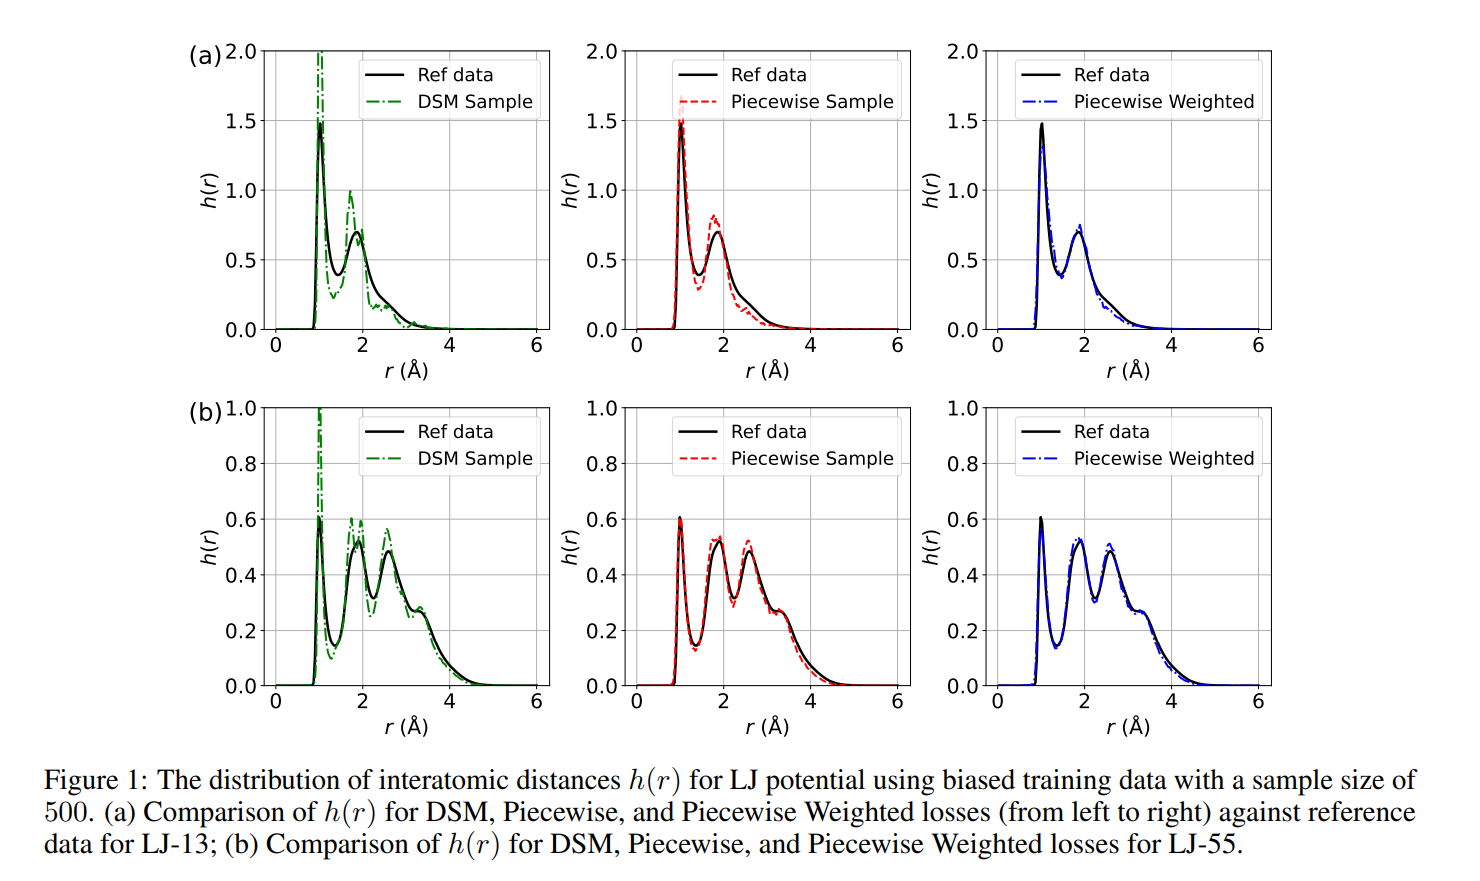
\includegraphics[width=0.8\textwidth]{../figures/psm0.png}
    \end{figure}
\end{frame}

\begin{frame}{Experiments on first 5, 000 frames for MD reference trajectories}
    \begin{figure}
        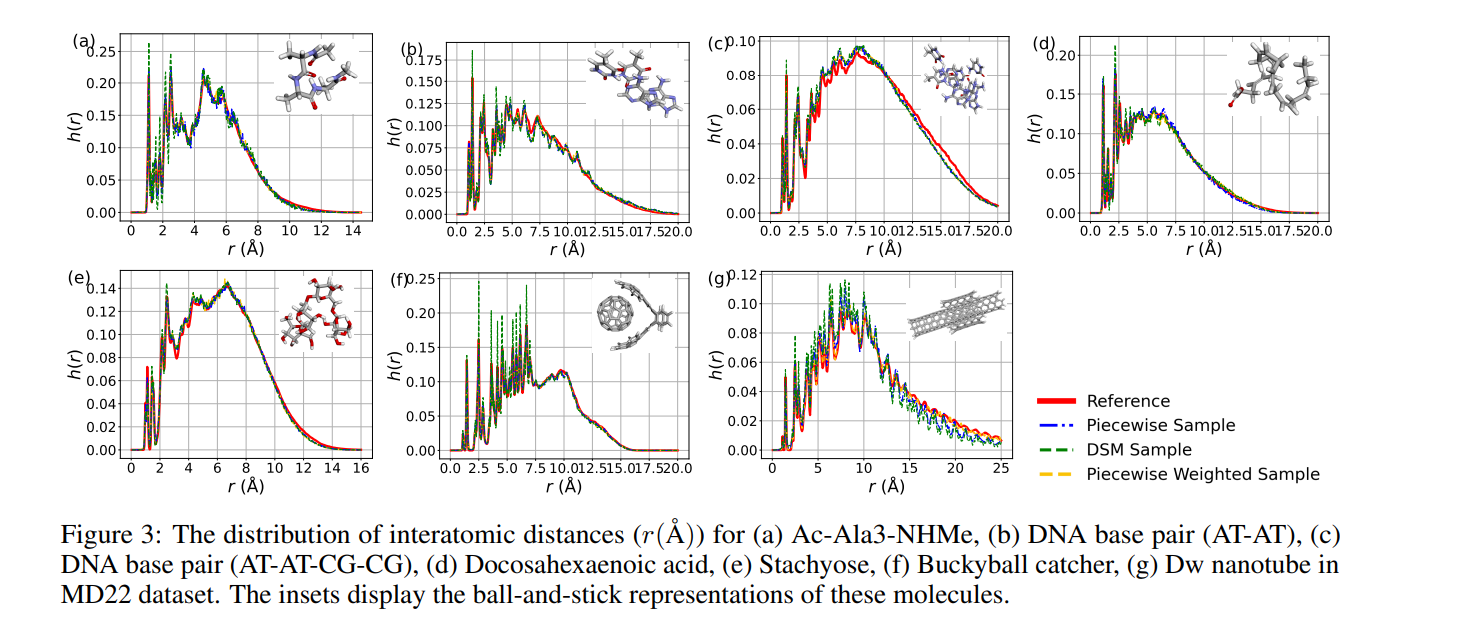
\includegraphics[width=0.9\textwidth]{../figures/psm.png}
    \end{figure}
\end{frame}

\section{Diffusion model: from theories to implementation}
\begin{frame}{From Theory to Practice}
Now that we have established the theoretical foundations of score matching and diffusion processes, let's explore how these concepts are implemented in practice through several key approaches:

\begin{itemize}
    \item \textbf{SMLD} (Score Matching Langevin Dynamics)
    \item \textbf{DDPM} (Denoising Diffusion Probabilistic Models)  
    \item \textbf{Continuous formulations} and their advantages
\end{itemize}

Each approach offers different insights into the practical implementation of diffusion-based generative models.
\end{frame}

\begin{frame}{SMLD}
    Score Matching Langevin Dynamic (SMLD) (Song, 2019) adding noise in a following manner
    \begin{equation}
        p(\Tilde{x}_i| x) = N(\Tilde{x}_i; x, \sigma_i^2)\equiv Ce^{-\frac{\|\Tilde{x}_i-x\|^2}{2\sigma_i^2}},
    \end{equation}
    where a geometric sequence $\sigma_1> \sigma_2>\cdots > \sigma_T \approx
    0$ is given to add noise with different level.

    In a random variable view, 
    \begin{equation}
        \Tilde{x}_i = x + \sigma_i \epsilon
    \end{equation}
    for different $\sigma_i$ to get different noised random variable $\Tilde{x}_i$.

    Training object $J_{DSM}$ is given by 
    \begin{equation}
        J_{DSM} = \frac{1}{2}\mathbb{E}_{\sigma_i}\mathbb{E}_{p(x)}\mathbb{E}_{p(\Tilde{x}_i|x)}\left[\|s_\theta(\Tilde{x}_i,\sigma_i)+\frac{\Tilde{x}_i-x}{\sigma_i^2}\|^2\right].
    \end{equation}

    Anneled Langevin MCMC for sampling 
    \begin{equation}
        x_t = x_{t-1} + \frac{\Delta t}{2}S_\theta(x_{t-1}) + \sqrt{\Delta t}\epsilon, \quad \epsilon\sim N(0,1).
    \end{equation}
\end{frame}

\begin{frame}{DDPM}
    denoising diffusion probabilistic models (DDPM) (Ho, 2020) 
    \begin{enumerate}
        \item Derived from the Evidence Lower BOund (ELBO), \textcolor{red}{Not} score matching.
        \item First provide adding noise and denoise in the forward and reverse process. 
    \end{enumerate} 

The main procedure
\begin{enumerate}
    \item Adding noise 
    \begin{equation}
        x_t = \sqrt{1-\beta_t}x_{t-1} +\sqrt{\beta_t}\epsilon;
    \end{equation}
    \item Transition kernel 
    \begin{equation}
        p(x_t|x_0) = N(x_t;\alpha_t x_0, \sigma_t^2),
    \end{equation}
    where $\alpha_t = \prod_{i=1}^{t} \sqrt{1-\beta_i}$ and $\sigma_t^2 = 1-\alpha_t^2$.
\end{enumerate}
\end{frame}

\begin{frame}{DDPM}
The main procedure (Continued)
\begin{enumerate}
    \item Adding noise 
    \begin{equation}
        x_t = \sqrt{1-\beta_t}x_{t-1} +\sqrt{\beta_t}\epsilon;
    \end{equation}
    \item Transition kernel 
    \begin{equation}
        p(x_t|x_0) = N(x_t;\alpha_t x_0, \sigma_t^2), \text{ i.e., } x_t = \alpha_t x_0 + \sigma_t \epsilon,
    \end{equation}
    where $\alpha_t = \prod_{i=1}^{t} \sqrt{1-\beta_i}$ and $\sigma_t^2 = 1-\alpha_t^2$.
    \item Training Loss
    \begin{equation}
        \mathbb{E}_{t\sim U[0,1]}\mathbb{E}_{p(x)}\mathbb{E}_{p(x_t|x)}\left[\|\epsilon_\theta(x_t,t)-\epsilon\|^2\right],
    \end{equation}
    where we have used the approximation
        $x_0 = \frac{x_t-\sigma_t\epsilon}{\alpha_t}$.
    \\[-1em]
    \item Sampling 
    \begin{equation}
        x_{t-1} = \frac{1}{\sqrt{1-\beta_t}}(x_t+\beta_t s_\theta(x_t, t)) +\sqrt{\beta_t}\epsilon_t, \quad t = T, T-1, \cdots, 1.
    \end{equation}
\end{enumerate}
\end{frame}

\section{Continuous version of Diffusion Model}

\begin{frame}{The continuous version of SMLD}
Recall that
\begin{equation}
    x_t = x_0 + \sigma_t\epsilon,
\end{equation}
we can prove that 
\begin{equation}
    x_t = x_{t-1} + \sqrt{\sigma_t^2-\sigma_{t-1}^2}\epsilon.
\end{equation}
\begin{proof}
    We can prove the formula by a Recurrence 
    \begin{equation}
    \begin{aligned}
        x_t &= x_{t-1} + \sqrt{\sigma_t^2-\sigma_{t-1}^2}\epsilon\\
        & = x_{t-2} + \sqrt{\sigma_{t-1}^2-\sigma_{t-2}^2}\epsilon +\sqrt{\sigma_t^2-\sigma_{t-1}^2}\epsilon\\
        & = x_{t-2} + \sqrt{\sigma_t^2-\sigma_{t-2}^2}\epsilon\\
        & = ...= x_0 + \sigma_t\epsilon, \quad \text{ where } \sigma_0\approx 0.
    \end{aligned}
    \end{equation}
\end{proof}
\end{frame}

\begin{frame}{The continuous version of SMLD}
From 
\begin{equation}
    x_t = x_{t-1} + \sqrt{\sigma_t^2-\sigma_{t-1}^2}\epsilon,
\end{equation}
we have 
\begin{equation}
    \begin{aligned}
        \Delta x_t &= \sqrt{\frac{\sigma_t^2-\sigma_{t-1}^2}{\Delta t}}\sqrt{\Delta t}\epsilon\\
        &= \sqrt{\frac{\sigma_t^2-\sigma_{t-1}^2}{\Delta t}}\Delta B_t.
    \end{aligned}
\end{equation}
Further, let $\Delta t\to 0$, we have
\begin{equation}
    dx = \sqrt{\frac{d\sigma_t^2}{d t}}dB_t.
\end{equation}
\end{frame}

\begin{frame}{The continuous version of DDPM}
Recall that 
\begin{equation}
        x_t = \sqrt{1-\beta_t}x_{t-1} +\sqrt{\beta_t}\epsilon.
\end{equation}
Similarly 
\begin{equation}
    \begin{aligned}
        x_t\approx (1-\frac{1}{2}\beta_t)x_{t-1} + \sqrt{\beta_t}\epsilon,
    \end{aligned}
\end{equation}
hence, we have
\begin{equation}
    \begin{aligned}
        \Delta x_t &= -\frac{1}{2}\Tilde{\beta_t} x_{t-1}\Delta t + \sqrt{\Tilde{\beta_t}}\sqrt{\Delta t}\epsilon, \quad \text{ where } \Tilde{\beta_t} = \frac{\beta_i}{\Delta t}\\
        & = -\frac{1}{2}\Tilde{\beta_t} x_{t-1}\Delta t + \sqrt{\Tilde{\beta_t}}\Delta B_t.
    \end{aligned}
\end{equation}
Further, let $\Delta t\to 0$, we finally obtain
\begin{equation}
    dx = -\frac{1}{2}\Tilde{\beta_t} x d t + \sqrt{\Tilde{\beta_t}}d B_t.
\end{equation}
\end{frame}

\begin{frame}{VE \& VP}
Summarizing the form of continuous DDPM and SMLD, we summarize the adding noise process as
\begin{equation}\label{eq:forward}
    dx = f(x, t)dt + g(t) dB_t,
\end{equation}
where the corresponding distribution $p(x, t)$ satisfying the following Fokker-Planck equation
\begin{equation}\label{eq:fp}
    \frac{\partial p(x,t)}{\partial t} + \nabla\cdot\left(f(x,t) p(x,t)\right) -\frac{1}{2}g^2(t) \triangle p(x,t)=0.
\end{equation}

Training DSM object 
\begin{equation}
    J_{DSM} = \mathbb{E}_{t\sim U[0,1]}\mathbb{E}_{p(x_0)}\mathbb{E}_{p(x_t|x_0)}\left[\|s_\theta(x_t,t)-\textcolor{red}{\nabla_{x_t}\log p(x_t|x_0)}\|^2\right].
\end{equation}
\end{frame}


\begin{frame}{VE \& VP adding noise}
To training the Denoising Score Match loss $J_{DSM}$ above, the key is to add noise by the transition kernel
\begin{equation}
    p(\Tilde{x}|x) \equiv p(x(t)|x(0)) = N(x(t); \Tilde{\alpha}_t x(0), \Tilde{\sigma}_t^2),
\end{equation}
from which we can obtain the noised data 
\begin{equation}
    x(t) = \Tilde{\alpha}_t x(0) + \Tilde{\sigma}_t\epsilon, \quad \epsilon\sim N(0,1).
\end{equation}

\textcolor{red}{The question becomes}: Given VE \& VP 
\begin{equation}
    dx = \sqrt{\frac{d[\sigma^2]}{dt}} dB_t,\quad 
    dx = -\frac{1}{2}\Tilde{\beta_t} x d t + \sqrt{\Tilde{\beta_t}}d B_t.
\end{equation}
how to derive $p(x(t)|x(0))$, i.e., $p(\Tilde{x}|x)$ for adding noise?
\end{frame}

\begin{frame}{VE \& VP Transition kernel}
The summarizing form of VE \& VP is 
\begin{equation}
    dx = h(t)xdt+ g(t)dB_t,
\end{equation}
where $h(t)=0$ for VE and $h(t)=-\frac{1}{2}\Tilde{\beta}(t)$ for VP. 

\begin{lemma}
Let $\mu(t) =\mathbb{E}[x(t)]$ and $\Sigma(t)=\mathbb{E}\left[(x-\mu(t))(x-\mu(t))^T\right]$, we have the following formula
\begin{equation}
\begin{aligned}
    \frac{d\mu(t)}{dt} = h(t)\mu(t),\quad
    \frac{d\Sigma(t)}{dt} = 2h(t)\Sigma(t)+g^2(t)I.
\end{aligned} 
\end{equation}
\end{lemma}
The proof of the Lemma can be found in a stochastic differential equation textbook such as Applied Stochastic Differential Equations, S\"{a}rkk\"{a} and Solin, 2019.
\end{frame}

\begin{frame}{VE \& VP Transition kernel}

\begin{lemma}
    For VE, the transition kernel is given by the following formula
\begin{equation}\label{eq:tranve}
    P(x(t)|x(0)) = N(x(t); x(0), \sigma^2(t)-\sigma^2(0)).
\end{equation}
For VE, 
\begin{equation}
    \Tilde{\alpha}_t \equiv  1, \quad \Tilde{\sigma}^2_t \equiv \sigma^2(t)-\sigma^2(0)\approx \sigma^2(t).
\end{equation}
\end{lemma}

\begin{lemma}
    For VP, the transition kernel is given the following formula
\begin{equation}\label{eq:tranvp}
    p(x(t)|x(0)) = N\left(x(t); x(0)e^{-\frac{1}{2}\int_0^t \Tilde{\beta}(s)ds},1-e^{-\int_0^t \Tilde{\beta}(s)ds}\right).
\end{equation}
For VP, 
\begin{equation}
    \Tilde{\alpha}_t \equiv  e^{-\frac{1}{2}\int_0^t \Tilde{\beta}(s)ds}, \quad \Tilde{\sigma}^2_t \equiv 1-e^{-\int_0^t \Tilde{\beta}(s)ds}.
\end{equation}
\end{lemma}
\end{frame}


\begin{frame}{Proof of VE transition kernel}
\begin{proof}
For VE, by a simple calculation we have

\begin{equation}
        \frac{d\mu(t)}{dt} = 0,\quad \frac{d\Sigma(t)}{dt} = \frac{d[\sigma^2(t)]}{dt},
\end{equation}
Hence, it is easy to obtain the following form 
\begin{equation}
        \mu(t) = \mu(0) = x(0),\quad \Sigma(t) = \sigma^2(t)-\sigma^2(0).
\end{equation}
Here we have used the fact  
\begin{equation}
    \mu(0) = x(0), \quad \Sigma(0)=0
\end{equation}
as $x(0)$ is taken as a constant, not a random variable.
And we obtain 
\begin{equation}
    P(x(t)|x(0)) = N(x(t); x(0), \sigma^2(t)-\sigma^2(0)).
\end{equation}
\end{proof}
\end{frame}

\begin{frame}{VP Proof: Differential Equations}
\begin{proof}
For VP, we have the differential equations:
\begin{equation}
    \frac{d\mu(t)}{dt} = -\frac{1}{2}\beta(t)\mu(t)
\end{equation}
\begin{equation}
    \frac{d\Sigma(t)}{dt} = -\beta(t)\Sigma(t)+\beta(t)
\end{equation}
We solve these using integrating factors.
\end{proof}
\end{frame}

\begin{frame}{VP Proof: Integrating Factors}
\begin{proofs}[\proofname\ (Cont)]
For the mean equation, multiply by $e^{\int_0^t\frac{1}{2}\beta(s)ds}$:
\begin{equation}
    \frac{d\mu(t)}{dt}e^{\int_0^t\frac{1}{2}\beta(s)ds} + \frac{1}{2}\beta(t)\mu(t) e^{\int_0^t\frac{1}{2}\beta(s)ds} =0
\end{equation}
For the variance equation, multiply by $e^{\int_0^t\beta(s)ds}$:
\begin{equation}
    \frac{d\Sigma(t)}{dt}e^{\int_0^t\beta(s)ds} +\beta(t)\Sigma(t)e^{\int_0^t\beta(s)ds} = \beta(t)e^{\int_0^t\beta(s)ds}
\end{equation}
\end{proofs}
\end{frame}

\begin{frame}{VP Proof: Solution}
\begin{proofs}[\proofname\ (Cont)]
This gives us:
\begin{equation}
    \frac{d}{dt} (\mu(t)e^{\int_0^t\frac{1}{2}\beta(s)ds}) = 0
\end{equation}
\begin{equation}
    \frac{d}{dt} (\Sigma(t)e^{\int_0^t\beta(s)ds}) = \frac{d}{dt} e^{\int_0^t\beta(s)ds}
\end{equation}
Solving with initial conditions $\mu(0) = x(0)$, $\Sigma(0) = 0$:
\begin{equation}
    p(x(t)|x(0)) = N\left(x(t); x(0)e^{-\frac{1}{2}\int_0^t \beta(s)ds},1-e^{-\int_0^t \beta(s)ds}\right)
\end{equation}
\end{proofs}
\end{frame}

\begin{frame}{Revisit adding noise}
The \textbf{equivalence} of the adding noise
\begin{enumerate}
    \item From the stochastic process, denote the variable $x_t$, we have 
    \begin{equation}
        d x_t = f(x,t)dt + g(t)dB_t, 
    \end{equation}
    with corresponding discrete form (Euler-Maruyama scheme)
    \begin{equation}
        x_{t+\Delta t} = x_{t} + f(x_t, t)\Delta t + g(t)\sqrt{\Delta t}\epsilon, \quad \epsilon\sim N(0, 1). 
    \end{equation}
\item From transition kernel perspective, 
\begin{equation}
    p(x_t) = \int_{x_0} p(x_0)p(x_t|x_0)dx_0,
\end{equation}
where 
\begin{equation}
    p(x_t|x_0) = N(x_t; \mu_t, \Sigma_t)=N(x_t; \Tilde{\alpha}_tx_0, \Tilde{\sigma}_t^2)=\frac{1}{C}e^{-\frac{\|x_t-\mu_t\|^2}{2\Sigma_t}}.
\end{equation}
\end{enumerate}

\end{frame}

\begin{frame}{Training recipe}
The training for VE follows the following process (VP is in a similar way)
\begin{enumerate}
    \item Random choose one data $x\sim p_{data}$;
    \item Random sample $t\sim U[0, 1]$;
    \item Random sample a white noise $\epsilon\sim N(0, 1)$;
    \item Adding noise 
    \begin{equation}
        x_t = \Tilde{\alpha}_t x + \Tilde{\sigma}_t\epsilon, 
    \end{equation}
    where the mean value $\Tilde{\alpha}_t x= x(0)$  and standard deviation $\Tilde{\sigma}_t = \sqrt{\sigma^2(t)-\sigma^2(0)}\approx \sigma(t)$ in VE referring to \eqref{eq:tranve}. VP is similar with the mean and standard deviation from its transition kernel \eqref{eq:tranvp};
    \item Compute the Loss
    by summation the following norm over $x$, $t$ and $\epsilon$ 
    \begin{equation}  
    \|s_\theta(x_t, t)-\epsilon/\Tilde{\sigma}_t\|.
    \end{equation} 
\end{enumerate}
\end{frame}


\begin{frame}{Inference: Reverse denoising process}
The reverse denoising process is given by 
\begin{equation}\label{eq:reverse}
    dx = (f(x,t)-g^2\nabla_x \log p(x,t))dt + g(t)dB_t,
\end{equation}
or 
\begin{equation}
    dx = (f(x,t)-\frac{1}{2}g^2\nabla_x \log p(x,t))dt,
\end{equation}
or 
\begin{equation}\label{eq:reverse2}
    dx = (f(x,t)-\frac{3}{2}g^2\nabla_x \log p(x,t))dt + \sqrt{2}g(t)dB_t,
\end{equation}
\begin{equation}
    \cdots
\end{equation}
Due to obeying the same Fokker-Planck equation for $p(x, t)$
\begin{equation}
    \frac{\partial p(x,t)}{\partial t} + \nabla\cdot(f(x,t) p(x,t)) -\frac{1}{2}g^2(t) \triangle p(x,t)=0.
\end{equation}
\end{frame}

\begin{frame}{Reverse Process Proof: Setup}
We prove the first reverse sampling form \eqref{eq:reverse}. The Fokker-Planck equation of the forward process \eqref{eq:forward} is:
\begin{equation}
    \frac{\partial p}{\partial t} + \nabla \cdot (f(x,t)p)-\frac{1}{2}g^2\triangle p = 0.
\end{equation}
Let $t = T-\tau$, we have:
\begin{equation}
    \frac{\partial p}{\partial \tau} - \nabla\cdot (f(x,T-\tau) p) + g^2\triangle p -\frac{1}{2}g^2\triangle p =0.
\end{equation}
\end{frame}

\begin{frame}{Reverse Process Proof: Derivation}
\begin{proofs}[\proofname\ (Cont)]
By $\nabla\cdot\nabla = \triangle$ and $\nabla \log p=\nabla p/p$:
\begin{equation}
    \frac{\partial p}{\partial \tau} - \nabla\cdot \bigg(\left(f(x,T-\tau)-g^2\nabla\log p\right)p\bigg) -\frac{1}{2}g^2\triangle p =0.
\end{equation}
Hence, we obtain the corresponding SDE form:
\begin{equation}
    dx = -(f(x, T-\tau)-g^2\nabla\log p)d\tau + gdB_\tau
\end{equation}
By substitution $\tau = T-t$:
\begin{equation}
    dx = (f(x,t)-g^2\nabla\log p)dt + gdB_t
\end{equation}
\end{proofs}
\end{frame}

% \begin{frame}{Interesting property about the ODE and SDE}
% \begin{enumerate}
%     \item The forward SDE and the reverse SDE has different sign 
% \end{enumerate}
% \end{frame}

\begin{frame}{Inference recipe}
The inference for VE follows the following process (VP is in a similar way)
\begin{enumerate}
    \item Random generate a noise at time $t=1$ as $x(1)\sim N(0, \sigma^2_{max})$;
    \item Integrate the reverse sampling equation 
    \begin{equation}
        dx = \left(f(x,t)-g^2(t) s_\theta(x,t)\right)dt + g(t)dB_t
    \end{equation} or 
    \begin{equation}
        dx = (f-\frac{1}{2}g^2 s_\theta)dt
    \end{equation}
    over the time span $[0, 1]$ to get $x(0)$.
    \item Corrector process: at each internal value $x(t)$, we can relax the value $x(t)$ by a corrector, which takes the Langevin MCMC process. 
\end{enumerate}

\end{frame}


\begin{frame}{The Corrector: revisit Langevin MCMC}
The Langevin diffusion process is given by 
\begin{equation}
    x_i = x_{i-1}+\frac{\Delta t}{2}\textcolor{red}{\nabla_x\log p(x_{i-1})}+\sqrt{\Delta t}\epsilon, \quad \epsilon\sim N(0, 1).
\end{equation}
We can prove   $\pi(x)$ of the obtained data points $\{x_i\}_{i=1}^N$ converges to $p(x)$.

\begin{proofs}
The continuous form of the scheme is:
\begin{equation}
    dx = \frac{1}{2}\nabla\log p(x) dt + dB_t.
\end{equation}
The corresponding Fokker-Planck equation is:
\begin{equation}
\frac{\partial\pi(x,t)}{\partial t} + \nabla\cdot(\frac{1}{2}\nabla\log p(x) \pi(x,t)) -\frac{1}{2}\triangle \pi(x,t) = 0.
\end{equation}
With sufficient time evolution, the distribution converges to a stable distribution where:
\begin{equation}
    \frac{\partial \pi(x,t)}{\partial t} = 0, \quad t\to \infty.
\end{equation}
\end{proofs}
\end{frame}

\begin{frame}{The Corrector: revisit Langevin MCMC}

\begin{proofs}[\proofname\ (Cont)]
Hence we have:
\begin{equation}
    \nabla\cdot(\pi\nabla\log p - \nabla\pi) = 0, \quad \forall x.
\end{equation}
Therefore:
\begin{equation}
    \nabla\log p = \nabla\log \pi
\end{equation}
given that $\pi>0$ almost everywhere. 
Hence:
\begin{equation}
    \pi^*(x) = p(x)
\end{equation}
where $\pi^*$ is the stable distribution of $\pi(x, t)$.
\end{proofs}
\end{frame}

\section{Mathematical motivation for Flow Matching}

\begin{frame}{Probability Path and Coupling}
\begin{itemize}
  \item Let $\{p_t\}_{t\in[0,1]}$ be a prescribed path of marginals on $\R^d$ with $p_0$ simple and $p_1$ the data.
  \item A \emph{coupling} induces random trajectories $t\mapsto \xt$ with instantaneous velocity $\xdot = \frac{\dd}{\dd t} \xt$ (may be stochastic given $\xt$).
  \item Goal: learn a \emph{deterministic} vector field $v:\R^d\times[0,1]\to\R^d$ such that the ODE
  \[
    \frac{\dd}{\dd t} x_t = v( x_t,t),\qquad  x_0\sim p_0,
  \]
  yields marginals $ x_t\sim p_t$ for all $t$.
\end{itemize}

\begin{remark}
    We can depict the flow matching and diffusion through the probability transition v.s. the trajectories. And also, we can connect the Neural ODE with the Flow matching.
\end{remark}

\end{frame}

% \begin{frame}{Distributions and Notation}
% \begin{itemize}
%   \item Denote the density of $\xt$ by $p_t(x)$, and the joint law of $(\xt,\xdot)$ by $\mu_t(\dd x,\dd \dot x)$ with conditional density $p(\dot x\given x,t)$.
%   \item Define the \emph{conditional-mean velocity}
%   \[
%     \vstar(x,t) \;:=\; \E[\xdot \mid \xt=x,\,t] \;=\; \int_{\R^d} \dot x \, p(\dot x\given x,t)\,\dd \dot x.
%   \]
% \end{itemize}
% \end{frame}

\begin{frame}{Strong and\ Weak Continuity}

From the Fokker--Planck equation, for $\frac{\dd x}{\dd t} = v(x,t)$, we have
\[
\pd_t p_t(x) + \nabla\!\cdot\!\big(p_t(x)\, v(x,t)\big)=0.
\]

The corresponding weak form of above strong form is

\begin{block}{Weak form (for any test functions $\ph\in C_c^\infty(\R^d)$)}
\[
\frac{\dd}{\dd t}\int_{\R^d} \ph(x)\,p_t(x)\,\dd x
\;=\; \int_{\R^d} \nabla \ph(x)\!\cdot\! v(x,t)\,p_t(x)\,\dd x,
\]
i.e., 
\[\frac{\dd}{\dd t}\,\E[\ph(\xt)]
= \E[\nabla \ph(\xt)\!\cdot\! v(x,t)].\]
\end{block}
\end{frame}

\begin{frame}{Weak Form from Random Trajectories}
Let $x_t$ be the coupled trajectory (not necessarily deterministic). For any test function $\phi\in C_c^\infty(\R^d)$,
we have
\[
\frac{\dd}{\dd t}\,\E[\ph(\xt)]
= \E[\nabla \ph(\xt)\!\cdot\! \xdot],
\] 
by the expectation of the derivative of the test function.

Expanding the expectation into integrals at a fixed $t$:
\begin{align*}
\E[\nabla \ph(\xt)\!\cdot\! \xdot]
&= \iint_{\R^d\times \R^d} \nabla\ph(x)\!\cdot\!\dot x \; \mu_t(\dd x,\dd \dot x) \\
&= \int_{\R^d} \nabla\ph(x)\!\cdot\!\Big(\int \dot x\, p(\dot x\given x,t)\,\dd \dot x\Big)\, p_t(x)\,\dd x \\
&= \int_{\R^d} \nabla\ph(x)\!\cdot\! \vstar(x,t)\, p_t(x)\,\dd x = \E[\nabla \ph(\xt)\!\cdot\! \vstar(x,t)].
\end{align*}
where $\vstar(x,t)\equiv\E[\xdot \mid \xt=x,\,t] = \int_{\R^d} \dot x\, p(\dot x\given x,t)\,\dd \dot x$.
Thus the random path induces the weak identity with $v=\vstar$.
\end{frame}

\begin{frame}{Theoretical Support: Conditional Expectation}
\begin{theorem}
\label{thm:conditional_expect_flow}
    Let $X$ be an integrable random variable. Then for each $\sigma$-algebra $\mathcal{V}$ and $Z \in \mathcal{V}$, $Z^* = \mathbb{E}(X| \mathcal{V})$ solves the least square problem %\cite{evans2012introduction}
    $$\text{argmin}_{Z\in \mathcal{V}} \| Z - X\|\,,$$
    where $\| Z\| = \left( \int Z^2 dP \right)^{\frac{1}{2}}$.
\end{theorem}

\begin{figure}
    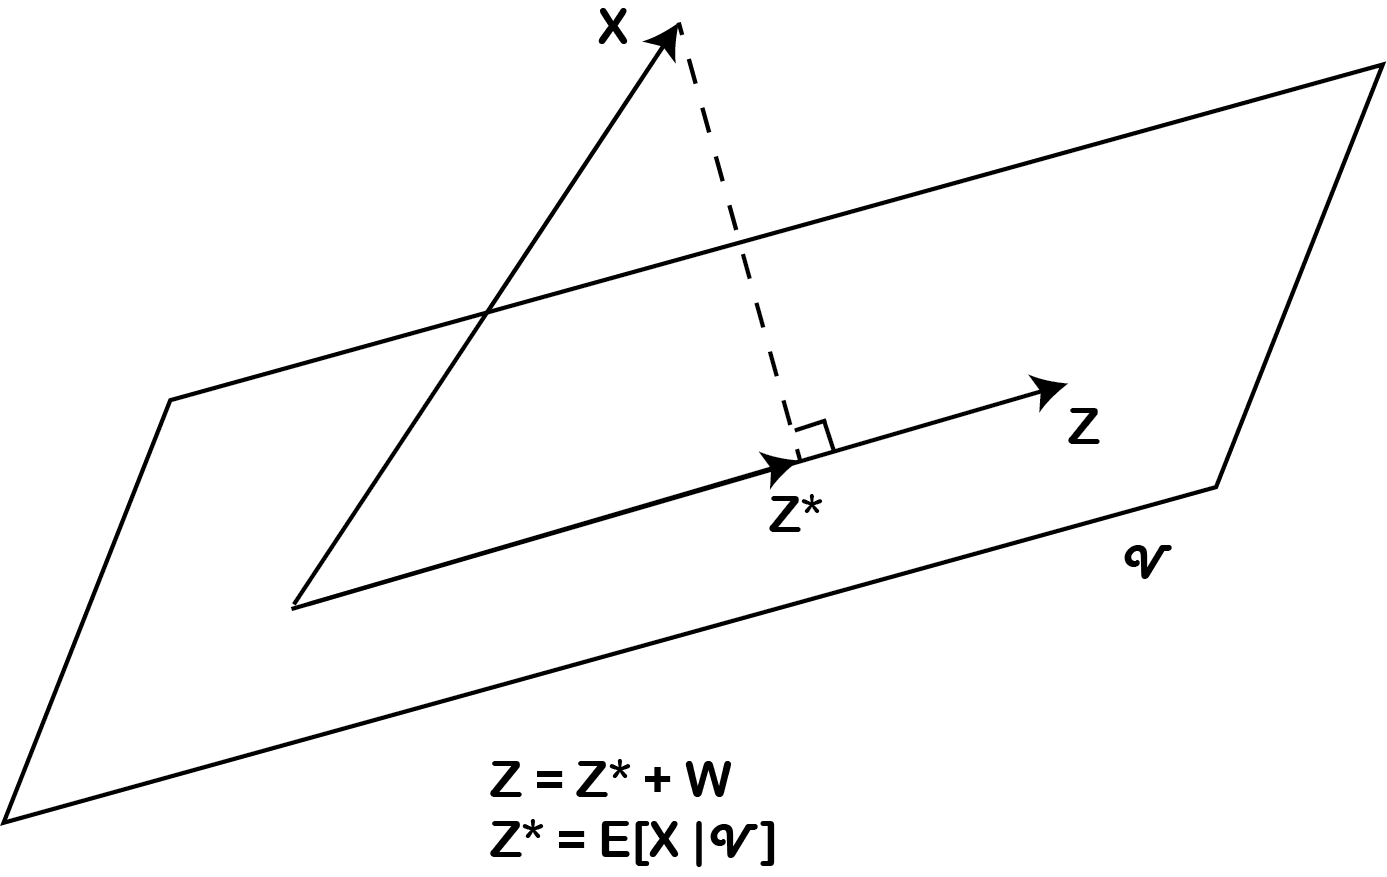
\includegraphics[width=0.3\textwidth]{../figures/conditional_expectation.png}
\end{figure}
Hence we have $L=\E\|v_\theta(\xt,t)-\xdot\|^2$.
\end{frame}

\begin{frame}{Practical Training Recipe (Per-Iteration)}
\begin{enumerate}
  \item Sample $t\sim w(t)$ (typically uniform on $[0,1]$).
  \item Sample $(\xt,\xdot)$ from the chosen path coupling.
  \item Regress $\xdot$ on $(\xt,t)$ via the MSE:
  \[
  \mathcal{L} = \big\| v_\theta(\xt,t) - \xdot \big\|^2.
  \]
  \item Update $\theta$ by SGD; no density estimation, no reverse simulation is needed during training.
\end{enumerate}
\begin{remark}
Different path/coupling choices change $\vstar$ and the irreducible variance $\E\|\xdot-\vstar\|^2$, affecting sample efficiency and optimization, but the optimal target remains the conditional mean.
\end{remark}
\end{frame}

\begin{frame}{Key Takeaways}
\begin{itemize}
  \item The correct notion of ``matching the path'' is the \textbf{weak continuity} identity for all test functions.
  \item The only deterministic field depending on $(x,t)$ that preserves this identity is the \textbf{conditional mean velocity}
  \[
  \boxed{\ \vstar(x,t)=\E[\dot x_t\mid x_t=x,\,t]\ }.
  \]
  \item The \textbf{flow-matching MSE} is precisely the $L^2$ projection selecting $\vstar$:
  \[
  v_\theta \;\xrightarrow[\text{minimize}]{\ \E\|v_\theta(\xt,t)-\xdot\|^2\ }\ \vstar.
  \]
\end{itemize}
\end{frame}

\section{Connection with Diffusion Models}

\begin{frame}{Fokker--Planck / Forward Kolmogorov}
\begin{theorem}[Fokker--Planck / Forward Kolmogorov]
Let $(X_t)_{t\ge 0}\in\mathbb{R}^N$ solve the It\^o SDE
\[
dX_t=\mu(X_t,t)\,dt+\boldsymbol{\sigma}(X_t,t)\,dW_t,
\]
where $\mu:\mathbb{R}^N\times[0,\infty)\!\to\!\mathbb{R}^N$ is the drift,
$\boldsymbol{\sigma}:\mathbb{R}^N\times[0,\infty)\!\to\!\mathbb{R}^{N\times M}$ the diffusion, and
$W_t$ an $M$-dimensional standard Wiener process. 
Define the diffusion tensor
\[
D(x,t)\coloneqq \frac{1}{2}\,\boldsymbol{\sigma}(x,t)\,\boldsymbol{\sigma}(x,t)^{\!\top}\in\mathbb{R}^{N\times N}.
\]
Then the (smooth) density $p(x,t)$ satisfies the Fokker--Planck equation
\[
\boxed{\;
\partial_t p(x,t)
= -\sum_{i=1}^N \frac{\partial}{\partial x_i}\big[\mu_i(x,t)\,p(x,t)\big]
\;+\;\sum_{i,j=1}^N 
\frac{\partial^2}{\partial x_i\,\partial x_j}\big[D_{ij}(x,t)\,p(x,t)\big]
\;}
\]
for $t>0$, with $p(x,0)=p_0(x)$.
\end{theorem}
\end{frame}

\begin{frame}{Isotropic diffusion: $\boldsymbol{\sigma}(x,t)=\sigma(t)\,\mathbf{I}_N$}
When $\boldsymbol{\sigma}(x,t)=\sigma(t)\,\mathbf{I}_N$, the diffusion tensor becomes
\[
D(x,t)=\tfrac{1}{2}\,\sigma(t)^2\,\mathbf{I}_N,
\qquad
D_{ij}(x,t)=\tfrac{1}{2}\,\sigma(t)^2\,\delta_{ij}.
\]
Hence the Fokker--Planck equation simplifies to the drift--diffusion form
\[
\boxed{\;
\partial_t p(x,t)
= -\nabla\!\cdot\!\big(\mu(x,t)\,p(x,t)\big)
\;+\;\frac{\sigma(t)^2}{2}\,\Delta p(x,t)
\;}
\]
where $\nabla\!\cdot(\mu p)=\sum_{i=1}^N \partial_{x_i}\!\big(\mu_i p\big)$ and $\Delta=\sum_{i=1}^N \partial_{x_i}^2$ is the Laplacian.
\end{frame}


\begin{frame}{Mathematical connection to diffusion models}
\textbf{Theoretical link}: For a forward SDE \(\dd\vx = f(\vx,t)\,\dd t + g(t)\,\dd B_t\), the probability flow ODE is:
\begin{equation}
    \frac{\dd}{\dd t}\,\vx = f(\vx,t) - \tfrac{1}{2}g^2(t)\,\grad_{\vx}\log p(\vx,t).
\end{equation}

\textbf{Key mathematical insight}: When Flow Matching uses Gaussian paths that match the SDE's marginal distributions \(p_t\), the learned velocity field \(\mathbf{v}_\theta\) approximates the probability flow drift:
\begin{equation}
    \mathbf{v}_\theta(\vx,t) \approx f(\vx,t) - \tfrac{1}{2}g^2(t)\,\grad_{\vx}\log p(\vx,t)
\end{equation}

\textbf{Crucial advantage}: Flow Matching achieves this approximation \emph{without} ever computing the score \(\grad_{\vx}\log p(\vx,t)\) during training!

\textbf{Practical implications}: This connection allows Flow Matching to inherit the theoretical guarantees of diffusion models while avoiding their computational bottlenecks.
\end{frame}

\begin{frame}{Mathematical derivation: probability flow ODE}
\textbf{Setup}: Forward SDE \(\dd\vx=f(\vx,t)\,\dd t + g(t)\,\dd B_t\) with density \(p(\vx,t)\) solving the Fokker-Planck equation:
\begin{equation}
    \partial_t p = -\grad\cdot(f p) + \tfrac{1}{2}g^2\,\triangle p.
\end{equation}

\textbf{Key insight}: A deterministic ODE \(\dot{\vx}=\mathbf{v}(\vx,t)\) transports densities via the continuity equation:
\begin{equation}
    \partial_t p + \grad\cdot(p\,\mathbf{v}) = 0.
\end{equation}

\textbf{Mathematical derivation}: Equating the two equations:
\begin{align}
    -\grad\cdot(p\,\mathbf{v}) &= -\grad\cdot(f p) + \tfrac{1}{2}g^2\,\triangle p\\
    \Rightarrow\; \mathbf{v} &= f - \tfrac{1}{2}g^2\,\frac{\grad p}{p} 
    \;=\; f - \tfrac{1}{2}g^2\,\grad\log p.
\end{align}

\textbf{Result}: The probability flow ODE drift is \(\mathbf{v} = f - \tfrac{1}{2}g^2\,\grad\log p\).

\textbf{Connection to Flow Matching}: When Flow Matching learns \(\mathbf{v}_\theta\), it approximates this probability flow drift without computing the score \(\grad\log p\).
\end{frame}


\begin{frame}{Questions}
    From 
        \begin{enumerate}
            \item Score model $s_\theta(x_t)\to s_{\theta^*}(x_t)\equiv\mathbb{E}[\nabla \log p(x_t|x_0)\mid x_t]$
            \item $X$ prediction model ( denoising model, $x0$ model) $x_\theta(x_t) \to x_{\theta^*}(x_t)\equiv \mathbb{E}[x_0\mid x_t]$;
            \item $\epsilon$ prediction model $\epsilon_\theta(x_t)\to\epsilon_{\theta^*}(x_t)\equiv\mathbb{E}[\epsilon\mid x_t]$.
        \end{enumerate}
    and 
    \[\vstar(x_t)=\E[\dot x_t\mid x_t]\],
    what is the relationship between optimal $v_\theta(x,t)$ and the above models?
    Hints:
    \begin{equation}
        v_{\theta^*}(x_t) = \E[\dot x_t\mid x_t] = \E[\dot{\alpha}(t)x_t + \dot{\sigma}(t)\epsilon\mid x_t].
    \end{equation}
    and 
    \begin{equation}
        s(x_t) = \mathbb{E}_x[\nabla_{x_t} \log p(x_t|x_0)| x_t]=\mathbb{E}_x[-\frac{x_t-\alpha x_0}{\sigma^2}| x_t] = -\frac{x_t-\alpha \mathbb{E}[x_0|x_t]}{\sigma^2}.
    \end{equation}
        
\end{frame}

\section{Conditional Paths and Velocity Targets}

\begin{frame}{Gaussian conditional paths: mathematical derivation}
\textbf{Assumption}: Gaussian conditional paths
\begin{equation}
    q_t(\vx\mid\vxz) = \mathcal{N}\big(\vx;\; \boldsymbol{\mu}_t(\vxz),\, \sigma_t^2\mathbf{I}\big),\quad \vxt = \boldsymbol{\mu}_t(\vxz) + \sigt\veps.
\end{equation}

\textbf{Mathematical derivation}: Taking the time derivative of the path:
\begin{equation}
    \frac{\dd}{\dd t}\,\vxt = \dot{\boldsymbol{\mu}}_t(\vxz) + \dot{\sigt}\,\veps,\quad \veps=\frac{\vxt-\boldsymbol{\mu}_t(\vxz)}{\sigt}.
\end{equation}

\textbf{Conditional expectation}: Since \(\veps\) is independent of \(\vxt\) given \(\vxz\), we have:

\begin{equation}
    \boxed{\;v = \dot{\boldsymbol{\mu}}_t(\vxz) + \frac{\dot{\sigt}}{\sigt}\Big(\vx-\boldsymbol{\mu}_t(\vxz)\Big).\;}
\end{equation}
\end{frame}

\begin{frame}{Mathematical analysis of path choices}
\textbf{1. Linear bridge} (optimal transport):
\begin{itemize}
    \item \(\boldsymbol{\mu}_t(\vxz)=(1-t)\,\vxz\), \(\sigt=t\,\sigma_{\max}\)
    \item \textbf{Mathematical property}: Minimizes Wasserstein-2 distance
    \item \textbf{Velocity}: \(v = \frac{\sigma_{\max}}{t}(\vx-\vxz)\)
    \item \textbf{Advantage}: Direct connection to optimal transport theory
\end{itemize}

\textbf{2. VP-like} (DDPM-inspired):
\begin{itemize}
    \item \(\boldsymbol{\mu}_t(\vxz)=\alpha(t)\,\vxz\), \(\sigt=\sqrt{1-\alpha^2(t)}\)
    \item \textbf{Mathematical property}: Preserves energy structure
    \item \textbf{Velocity}: \(v = \dot{\alpha}(t)\vxz + \frac{\dot{\sigt}}{\sigt}(\vx-\alpha(t)\vxz)\)
    \item \textbf{Advantage}: Compatible with existing diffusion model schedules
\end{itemize}

\textbf{3. VE-like} (SMLD-inspired):
\begin{itemize}
    \item \(\boldsymbol{\mu}_t(\vxz)=\vxz\), \(\sigt=\sigma(t)\) increasing
    \item \textbf{Mathematical property}: Preserves data structure
    \item \textbf{Velocity}: \(v = \frac{\dot{\sigma}(t)}{\sigma(t)}(\vx-\vxz)\)
    \item \textbf{Advantage}: Simple form, good for high-dimensional data
\end{itemize}

\textbf{Key insight}: All choices provide \emph{closed-form} \(\mathbf{u}_t\) via the boxed formula!
\end{frame}

\begin{frame}{Derivation: VE/VP target forms}
\small
\textbf{VE-like.} \(\boldsymbol{\mu}_t(\vxz)=\vxz\), \(\sigt=\sigma(t)\). Then
\begin{equation}
    v = 0 + \frac{\dot\sigt}{\sigt}\,(\vx-\vxz).
\end{equation}
\textbf{VP-like.} \(\boldsymbol{\mu}_t(\vxz)=\alpha(t)\,\vxz\), \(\sigt=\sqrt{1-\alpha^2(t)}\). Using
\(\mathbf{u}_t=\dot{\boldsymbol{\mu}}_t + (\dot\sigt/\sigt)(\vx-\boldsymbol{\mu}_t)\), we get
\begin{align}
    v
    &= \dot\alpha\,\vxz + \frac{\dot\sigt}{\sigt}\,\vx - \frac{\dot\sigt}{\sigt}\,\alpha\,\vxz\\
    &= \frac{\dot\sigt}{\sigt}\,\vx + \Big(\dot\alpha - \alpha\,\frac{\dot\sigt}{\sigt}\Big)\,\vxz.
\end{align}
No explicit form for \(\dot\sigt/\sigt\) is required to train; schedules determine it numerically.

\textbf{Mathematical insight}: These derivations show how different path choices lead to different velocity field structures, all computable analytically.
\end{frame}

\section{Flow Matching Training and Inference}

\begin{frame}{Flow Matching: mathematical training objective}
\textbf{Theoretical foundation}: Given conditional paths \(q_t(\vx\mid\vxz)\), the optimal velocity field satisfies:
\begin{equation}
    \vstar(x,t)=\E[\dot x_t\mid x_t=x,\,t]
\end{equation}

\textbf{Training procedure}:
\begin{enumerate}
    \item Sample \(t\sim\mathcal{U}[0,1]\), \(\vxz\sim p_{\text{data}}\), \(\vxt\sim q_t(\cdot\mid\vxz)\)
    \item Compute analytic target \(\mathbf{u}_t(\vxt\mid\vxz)\) from chosen path
    \item Minimize regression loss
\end{enumerate}

\textbf{Mathematical objective}:
\begin{equation}
    J_{\text{FM}} = \EE\big[\,\|\, \mathbf{v}_\theta(\vxt,t) - v\,\|^2\,\big].
\end{equation}

\textbf{Key mathematical advantage}: No score estimation needed; all targets are analytic!

\textbf{Computational benefits}:
\begin{itemize}
    \item Stable gradients (no exploding/vanishing)
    \item Parallelizable across time steps
    \item No special architectural requirements
\end{itemize}
\end{frame}

\begin{frame}{Mathematical foundation of inference}
\textbf{Theoretical basis}: The learned velocity field \(\mathbf{v}_\theta(\vx,t)\) defines a deterministic ODE:
\begin{equation}
    \frac{\dd}{\dd t}\,\vx = \mathbf{v}_\theta(\vx,t), \quad t\in[0,1]
\end{equation}

\textbf{Mathematical properties}:
\begin{itemize}
    \item \textbf{Existence}: Under Lipschitz conditions, solutions exist and are unique
    \item \textbf{Consistency}: The ODE preserves the continuity equation
    \item \textbf{Stability}: Deterministic integration avoids accumulation of stochastic errors
\end{itemize}

\textbf{Generation process}:
\begin{enumerate}
    \item Initialize \(\vx(1)\sim p_1\) (e.g., \(\mathcal{N}(0,\mathbf{I})\))
    \item Integrate ODE backwards: \(\frac{\dd}{\dd t}\,\vx = \mathbf{v}_\theta(\vx,t)\), \(t:1\to 0\)
    \item Use standard ODE solvers (Euler, RK4, Dormand-Prince, etc.)
\end{enumerate}

\textbf{Mathematical advantages}:
\begin{itemize}
    \item Deterministic sampling (reproducible)
    \item Fast with large solver steps
    \item No stochastic correctors needed
\end{itemize}
\end{frame}



\begin{frame}{Welcome inputs}  
  \centering  
  Any comments?
  \\[2em]
  Welcome your inputs!  
\end{frame}  
  
\end{document}  
